\chapter{Deceptive Box: PANDA meets evasive malware}
\label{chap:4}

The idea of this thesis was to develop a plugin to modify the Virtual Machine and hide execution artifacts from the system. In this way Evasive Malware can be run on the system having them to reveal the real capabilities by tricking them into believing that the system running is a real physical system.
\todo{More general details}

\section{Leveraging panda-re to hide artifacts from the system}

As widely discussed in the previous chapters \textbf{PANDA} provides many useful features that can be used to modify a running virtual machine. The important thing is to hide artifacts from a very specific process, the evasive malware, and therefore the plugin allows to specify a process name that should be targeted. Instead of hiding every single artifacts left by QEMU on the system it was preferred to analyze the most common checks and focus on those, subsequently, the plugin can be extended to support different evasion techniques. Due to the nature of this project the resulting plugin will need to be run both on live and replay modes. As a matter of fact deep modifications of the system are required in order to hide unwanted strings and behaviour and fool the malware.

Some of the hardware based checks can be avoided simply by fine tuning the system, in particular the disk size and RAM size can be adjusted to avoid the detection by setting the RAM to a value greater that 1 GB and the disk to a size greater than 60GB. 

It was decided in the beginning to write a C plugin in order to perform all the evasive countermeasures and keep the overhead low. However, this quickly turned out to be unfeasible as some of the plugins required to correctly mask virtualization artifacts are designed to be used with the python interface. It is the case of hooks.

The main idea was to use Paranoid Fish and Al-khaser to test what would be detected on the machine and then later patch the relevant artifacts to let the system "pass that check". 

The \textbf{PANDA} plugins directly used for this project are: 

\begin{itemize}
    \item \textbf{osi} or Operating System Introspection was used to access some of the internal structures of Windows. The peculiarity of this plugin is that it puts a layer of abstraction on top of the Operating System making it easy to write a plugin that will then work on all the supported OS. 
% +-------------------+  +-------------------+
% |    Your Plugin    |  |    Your Plugin    |
% +-------------------+  +-------------------+
% |        osi        |  |        osi        |
% +-------------------+  +-------------------+
% |     osi_linux     |  |    win7x86intro   |
% +-------------------+  +-------------------+
    \item \textbf{syscalls2} is a plugin that provides a Plugin to Plugin interface each time a system call is executed. This plugin uses osi under the hood to perform system calls hooking, this allows for a breakpoint to be placed either when the syscall is executed or when the execution returns from the above sytem call. This latter part is particularly useful when exploring or changing the information returned from a specific syscall.
    
    \item \textbf{hooks} is a plugin that allows the user to specify a address and a function, the function will then be called each time that specific address is reached. This is essentially what a breakpoint is in a debugger.
    
\end{itemize}

Newer versions of windows are not supported by many of these plugins therefore in order to perform the analysis it was decided to use a 32 bit version of Windows 7.


\subsection{First Step: writing a C plugin}

The first approach was to write a \textbf{PANDA} plugin to hook system calls associated with typical footprinting performed by evasive malware. This involve having a deep understanding of how the Operating System works and which are its internal structures. A common source of information is the windows registry, there are 3 system calls that are used to access the registry: \lstinline{NtQueryValueKey, NtOpenKey} and \lstinline{NtEnumerateKey}. 

Using the \textbf{syscalls2} plugin different breakpoints were placed on the above mentioned system calls, in particular it was decided to capture the data returned by the above mentioned system calls. As \textbf{PANDA} is based on QEMU  \lstinline{NtEnumerateKey} and \lstinline{NtOpenKey} are useful to catch enumeration however, \lstinline{NtQueryValueKey} is the function that provides the final string used for detection.

\lstinline{NtQueryValueKey} is the user mode version of \lstinline{ZwQueryValueKey}. This function allows to query the content of a value inside a specific registry key. In particular the key to be queried must have been accessed before with the \lstinline{NtCreateKey} or \lstinline{ZwOpenKey}, these functions will return a \textit{KeyHandle} that identify that specific key and that must be passed as parameter to the \lstinline{NtQueryValueKey} function. In addition to this there are some other values required to properly query the registry key, in particular \textit{ValueName} holds the name of the value to be queried. \textit{KeyValueInformationClass} specify the type of information to be returned and Length specify the length of the output buffer called \textit{KeyValueInformation}. The complete header of such function can be seen in Figure \ref{fig:querykey}.

\begin{figure}[htp]
\centering
\begin{lstlisting}[language=C]
NtQueryValueKey(
  IN HANDLE               KeyHandle,
  IN PUNICODE_STRING      ValueName,
  IN KEY_VALUE_INFORMATION_CLASS KeyValueInformationClass,
  OUT PVOID               KeyValueInformation,
  IN ULONG                Length,
  OUT PULONG              ResultLength );
\end{lstlisting}
\caption{\lstinline{NtQueryValueKey} header}
\label{fig:querykey}
\end{figure}

The \textit{KeyValueInformationClass} is particularly interesting as based on this value the tyupe of information returned inside the \textit{KeyValueInformation} changes.

A common enumeration technique consists of querying the value \textit{SystemBiosVersion} which is found under the path \lstinline{HKEY_LOCAL_MACHINE\HARDWARE\Description\System} and comparing it with the string \textit{BOCHS}.

In order to patch the above described System Call using \textbf{PANDA} it was necessary to hook the function when it returns, this can be done in the C plugin by registering to use appropriate \textbf{PPP} callback in the \lstinline{init_plugin} section. The implementation can be seen in Figure \ref{fig:pinit}.

\begin{figure}[htp]
\centering
\begin{lstlisting}[language=C]
bool init_plugin(void *self) {
    panda_require("syscalls2");
    [...]
    PPP_REG_CB("syscalls2", on_NtQueryValueKey_return, NtQueryValueKey_return);
    [...]
    return true;
}
\end{lstlisting}
\caption{Snippet of code representing how to hook the \lstinline{NtQueryValueKey} function.}
\label{fig:pinit}
\end{figure} 

The above snippet of code will run the \lstinline{NtQueryValueKey_return} function every time the \lstinline{NtQueryValueKey} returns, it is therefore necessary to have specific checks in place in order to patch the system only when the system call is executed from within a specified program. This has been implemented with a check on the program name or on the PID. Details of the patching function can be seen in Figure \ref{fig:pfun}. The function, after checking if the program running is the one specified for analysis, checks if the queried value is \textit{SystemBiosVersion} then if the value corresponds to \textit{BOCHS} it will replace it with \textit{INTEL}. It is important to note that all the particular structures used by this functions had to be ported from the windows library to this plugin in order for them to be used. Moreover the \lstinline{guest_wstrncpy} function is a helper function used to copy strings from the memory as it can be seen in \ref{fig:gstrin}.

\begin{figure}[htp]
\centering
\begin{lstlisting}[language=C]
void NtQueryValueKey_return(
    CPUState* cpu,
    target_ulong pc,
    uint32_t KeyHandle,
    uint32_t ValueName, 
    uint32_t KeyValueInformationClass,
    uint32_t KeyValueInformation,
    uint32_t Length, 
    uint32_t ResultLength 
    ){ 
    if (check_pid(cpu, tpid, tname)){
        char *name;
        UNICODE_STRING vname;
        name = malloc(1024*sizeof(char));
        panda_virtual_memory_rw(cpu, ValueName, (uint8_t *)&vname, sizeof(UNICODE_STRING), 0); // extract the pointer to string
        guest_wstrncpy(cpu, name, 1024, vname.Buffer); // read the string
        if (strcmp(name, "SystemBiosVersion")==0){
            KEY_VALUE_PARTIAL_INFORMATION rr;
            panda_virtual_memory_rw(cpu, KeyValueInformation, (uint8_t *)&rr, Length, 0);
            if (rr.Data[0]=='B' && rr.Data[8] == 'S'){
                // printf("\n\tPatching BOCHS\n");
                for(int i=0;i<5;i++){
                    char sub[6] = "INTEL";
                    rr.Data[(i*2)] = sub[i];
                }
                panda_virtual_memory_rw(cpu, KeyValueInformation, (uint8_t *)&rr, Length, 1);    
            }
        }
        free(name);
        return;
    }
}
\end{lstlisting}
\caption{Patching the value inside the registry using the \lstinline{NtQueryValueKey_return} function.}
\label{fig:pfun}
\end{figure} 

\begin{figure}[htp]
\centering
\begin{lstlisting}[language=C] 
uint32_t guest_wstrncpy(CPUState *cpu, char *buf, size_t maxlen, target_ulong guest_addr) {
    buf[0] = 0;
    unsigned i;
    for (i=0; i<maxlen; i++) {
        panda_virtual_memory_rw(cpu, guest_addr + 2 * i, (uint8_t *)&buf[i], 1, 0);
        if (buf[i] == 0) {
            break;
        }
    }
    buf[maxlen-1] = 0;
    return i;
}
\end{lstlisting}
\caption{\lstinline{guest_wstrncpy} function implementation.}
\label{fig:gstrin}
\end{figure}

This is an effective method to patch various system calls and can easily be expanded for any other syscall used for Virtualization detection.


\subsection{Second Step: writing a python simulation}

Patching other virtualization artifacts such as library calls and CPUID instructions is a more complex task as there are no available plugins that perform the same task as the syscall2. It was therefore decided to switch to python this, as mentioned before, has some other advantages such as the ability to run a complete simulation by having complete control over the virtual machine from the python script. Moreover one of the advantages of the python library is that it has a builtin mechanism for detecting the program that is running simply by passing its name to the python function, removing the need to implement a custom function as it has been done with the C plugin.

It must be noted that all the flexibility that python provides on the management and interaction side is at the cost of performance therefore simulations run using the python script have a much lower performance than the native ones. Moreover as cited before in order for the \textbf{PANDA} plugins to work it is necessary to use QEMU without the KVM acceleration, this further lowers the performance of the system. 

Pypanda uses Python decorators\footnote{\url{https://wiki.python.org/moin/PythonDecorators}} to implement callbacks and PPP functions, a decorator is a way of altering the functionality of functions, methods or classes without having to directly interact with the source code and avoiding repetitions. In Python decorators are defined with the \lstinline{@} symbol at the beginning of the line, the following function will then alter, replace or extend the one specified after the \lstinline{@}. In this particular case decorators let the user specify the function that should be run when the event defined by the callback happens. 

One of the detection techniques involve taking advantage of the information provided by the CPUID instruction as detailed in Section \ref{sec:evmal}. This particular instruction has a well defined callback in \textbf{PANDA} as it is used also by the taint plugin to perform actions inside the guest. The callback triggered by this instruction is \lstinline{PANDA_CB_GUEST_HYPERCALL}, the function implementing this callback should return \textit{True} if the hypercall is "processes", meaning that the plugin has already computed the result of CPUID, and \textit{False} otherwise. If the value returned is \textit{True} then the execution of the real CPUID instruction is skipped.

This allowed to write a function that reads the various parameters that CPUID takes as input in EAX and then acts accordingly. The function can be seen in Figure \ref{fig:cpuidpat}, when the value of EAX is one the function will simply replace the output of the instruction in ECX with the value 0. This did not pose any problem during the simulation however if the malware needs any of the other information available in the ECX registry this logic can quickly be modified by xor-ing the content of ECX, after it is populated by CPUID, with 0x80000000 (\lstinline{panda.arch.set_reg(cpu, "ECX", ecx^0x80000000)}). In the same way the relevant registers are zeored also for the other options.

\begin{figure}[htp]
\centering
\begin{lstlisting}[language=Python] 
@panda.cb_guest_hypercall(name="hyper", procname=process_name)
def tt(cpu):
    eax = panda.arch.get_reg(cpu, "EAX")
    if eax == 1:
        print("CPUID 0x1")
        panda.arch.set_reg(cpu, "ECX", 0) # the endianess is swapped (?)
        return True
    elif eax == 0x40000000:
        print("CPUID Vendor")
        panda.arch.set_reg(cpu, "ECX",0)
        panda.arch.set_reg(cpu, "EDX",0)
    elif eax >= 0x80000002 and eax<=0x80000004:
        print("CPUID Brand")
        panda.arch.set_reg(cpu, "EAX",0)
        panda.arch.set_reg(cpu, "EBX",0)
        panda.arch.set_reg(cpu, "ECX",0)
        panda.arch.set_reg(cpu, "EDX",0)
        return True
    return False
\end{lstlisting}
\caption{CPUID patching}
\label{fig:cpuidpat}
\end{figure}

The second part of the python plugin is a bit more complicated as it requires to hooks some specific functions in a library on the system. As the libraries are loaded at a different address each time it is necessary to first find out the right address at which the library will be loaded, then the offset of the function to be hooked must be added to the base address of library and finally it is possible to set the desired breakpoint. However, it must be noted that in order for the breakpoint to work the code of the library must have been already loaded in memory. 

In order to find the base address of the libraries loaded in the system it is possible to use the pypanda helper function \lstinline{panda.get_mappings(cpu)}, this is based on the osi plugin and will return as output a dictionary containing the 
libraries loaded in the system in that precise moment. This implies that if the function is called while a given executable is running it will return the libraries loaded by that executable. 

The function patched by the plugin are contained inside the \textit{kernel32.dll} library although the process is identical for any other library. In order to place the hook in the correct place it is important to first find out the offset of the function that will be hooked inside the library, this can be easily accomplished by opening the dll with pestudio which will give the offset of all the functions exported by the dll as it can be seen in Figure \ref{fig:pestudio}. 

\noindent
\begin{figure}[htp]
\centering
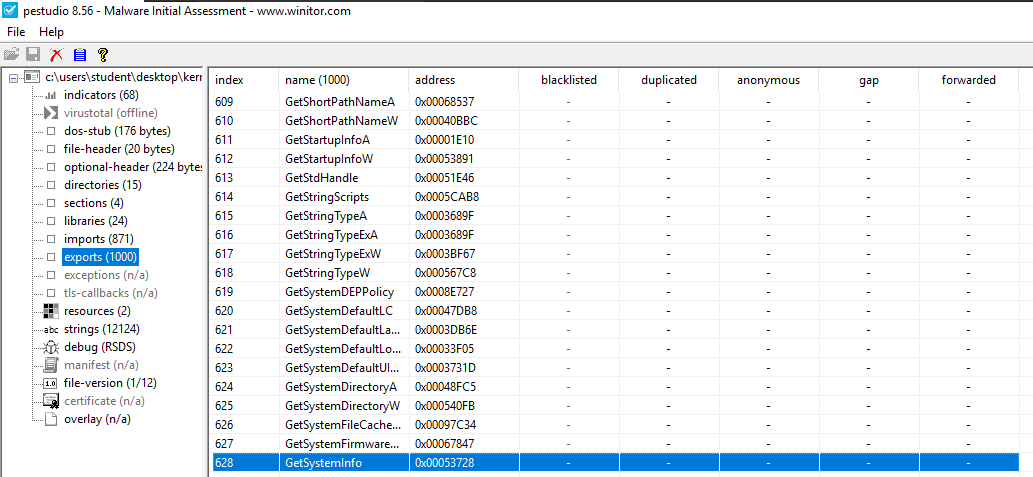
\includegraphics[width=\linewidth]{images/pestudio.png}
\caption{Finding offset of functions using pestudio}
\label{fig:pestudio}
\end{figure}

Subsequently in order to find the base address at which \textit{kernel32.dll} is loaded it is possible to place a breakpoint on the \lstinline{NtMapViewOfSection} system call using the syscalls2 plugin. The mentioned system call is used by a process to map a file into its memory address space, therefore each time a library is loaded a custom function will be called. This function, detailed in Figure \ref{fig:ntmap}, is then responsible to check if the loaded library corresponds to the one in which the function to be hooked resides. Once a match is found the function will in turn enable a memory callback (\lstinline{PANDA_CB_VIRT_MEM_BEFORE_READ}) and then disable itself.

\begin{figure}[htp]
\centering
\begin{lstlisting}[language=Python] 
@panda.ppp("syscalls2", "on_NtMapViewOfSection_return", name="ntmap")
def ntmap(cpu, pc, SectionHandle,  ProcessHandle, BaseAddress, ZeroBits, CommitSize, SectionOffset, ViewSize, InheritDisposition, AllocationType, Win32Protect):
    proc = panda.get_process_name(cpu)
    #print("PC 0x{:x}".format(pc))
    print(proc)
    if proc == process_name:
        mappings = panda.get_mappings(cpu)
        for mapping in mappings:
            print(
                "Name: "+ffi.string(mapping.name).decode(),
                "Base: 0x{:x} Size: 0x{:x}".format(mapping.base,mapping.size)
            )
            if ffi.string(mapping.name).decode().lower() == "kernel32.dll":
                global base
                base = mapping.base
                global si
                si = mapping.size
                print("Enabling memory callback")
                panda.enable_callback("cb1")
                print("Enabling hypercall callback")
                panda.enable_callback("hyper")
                print("Disabling MapViewOfSections hook")
                panda.disable_ppp("ntmap")
\end{lstlisting}
\caption{\lstinline{NtMapViewOfSection} hooking}
\label{fig:ntmap}
\end{figure}

The memory callback is necessary as when the \lstinline{NtMapViewOfSection} function is called the library is not yet loaded into the reserved virtual memory and therefore placing an hook at an address in that range will not work as it will be overwritten when the content of the dll is loaded. Instead by monitoring the reserved portion of memory for a read operation we will be sure that when the read takes place the code will have been loaded in memory. 

\todo{Finish this up, more details on rest of the python plugin}

\section{Results}

\todo{How the plugins helped compared to plain executon?}
